\chapter{SYSTEM DESIGN}

\section{System Architecture}
The system follows a typical \textbf{Client-Server Architecture} with a decoupled frontend and backend. The React frontend communicates with the Python (FastAPI) backend via RESTful APIs. The backend handles business logic, communicates with the Google Gemini API for NLP tasks, and interacts with the Supabase PostgreSQL database for data persistence.

% Placeholder for Diagram
\begin{figure}[H]
    \centering
    % \includegraphics[width=0.8\textwidth]{images/architecture_diagram.png}
    \caption{System Architecture Diagram}
    \label{fig:architecture}
\end{figure}

\section{Use Case Diagram}
The Use Case diagram illustrates the interactions between the primary actor (End User) and the system.

% Placeholder for Diagram
\begin{figure}[H]
    \centering
    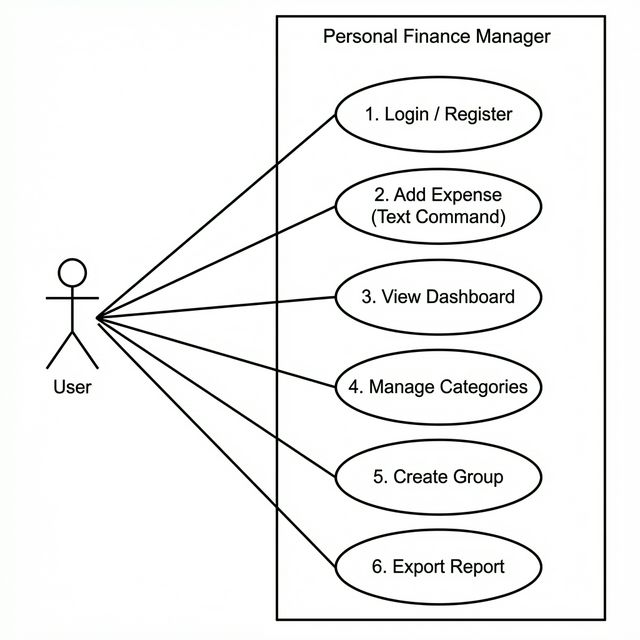
\includegraphics[width=0.8\textwidth]{images/use_case_diagram.png}
    \caption{Use Case Diagram}
    \label{fig:usecase}
\end{figure}

\section{Class Diagram}
The Class Diagram depicts the structure of the system's classes, their attributes, and relationships.

% Placeholder for Diagram
\begin{figure}[H]
    \centering
    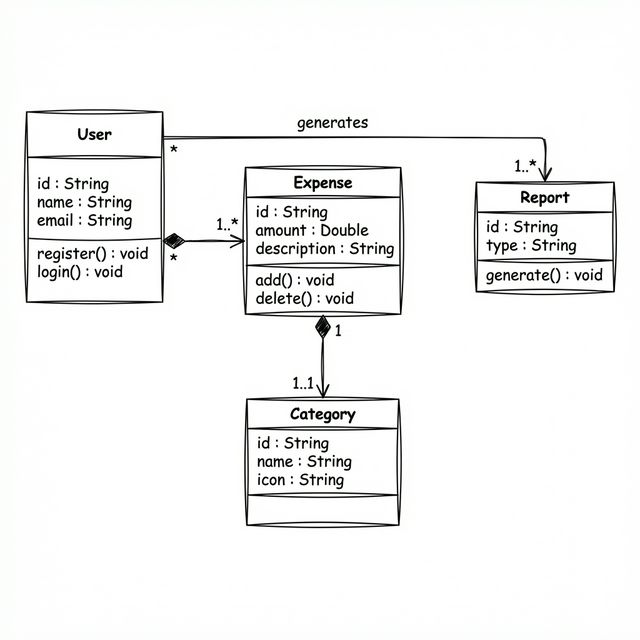
\includegraphics[width=0.8\textwidth]{images/class_diagram.png}
    \caption{Class Diagram}
    \label{fig:class}
\end{figure}

\section{Sequence Diagram}
The Sequence Diagram for the "Add Expense" feature shows the flow of messages between objects.

% Placeholder for Diagram
\begin{figure}[H]
    \centering
    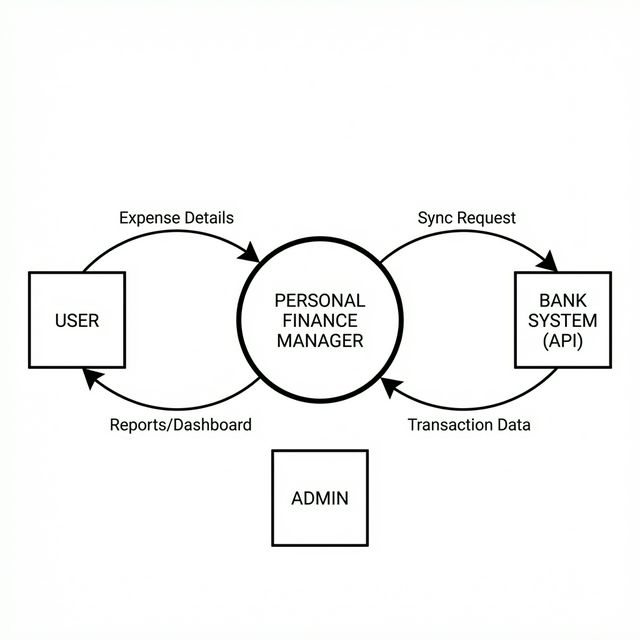
\includegraphics[width=0.8\textwidth]{images/sequence_diagram.png}
    \caption{Sequence Diagram}
    \label{fig:sequence}
\end{figure}

\section{Activity Diagram}
The Activity Diagram illustrates the workflow of adding an expense.

% Placeholder for Diagram
\begin{figure}[H]
    \centering
    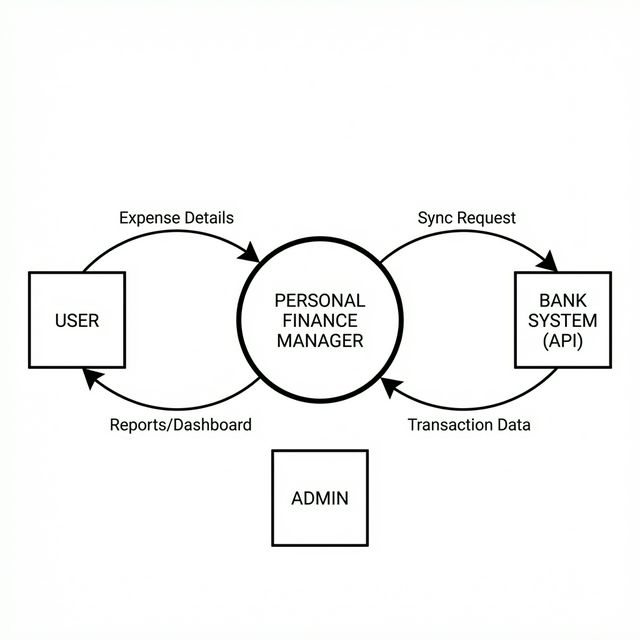
\includegraphics[width=0.8\textwidth]{images/activity_diagram.png}
    \caption{Activity Diagram}
    \label{fig:activity}
\end{figure}

\section{Database Design (ER Diagram)}
The Entity-Relationship (ER) diagram shows the database schema.

% Placeholder for Diagram
\begin{figure}[H]
    \centering
    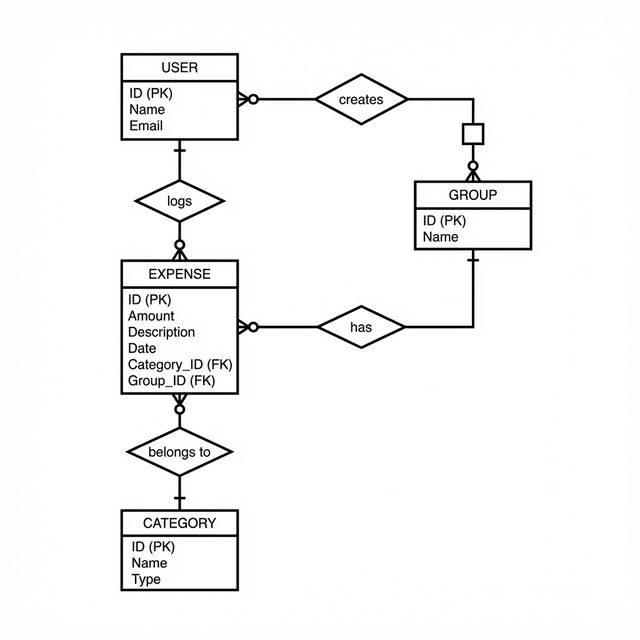
\includegraphics[width=0.8\textwidth]{images/er_diagram.png}
    \caption{Entity Relationship (ER) Diagram}
    \label{fig:er}
\end{figure}

\section{UI/UX Design}
The user interface was designed with a "Mobile First" approach, ensuring strict adherence to responsive design principles.
\begin{itemize}
    \item \textbf{Color Palette:} A clean, minimal color scheme (using TailwindCSS defaults) with distinct colors for income (green) and expense (red).
    \item \textbf{Typology:} Sans-serif fonts for readability (Inter/Roboto).
    \item \textbf{Interaction:} Smooth transitions and loading states for AI operations.
\end{itemize}
